% !tex root = ../Thesis.tex

This chapter describes the design, module implemetation and final implemetations
of the pitch correction system. The implementation code was written in Octave, a
free and open source alternative to Matlab. Some important, short code-snips are
shown and explaind to give deeper insight into the details of the implementation.

Since one of the goals of this report is to compare the performance of the pitch
corrector when using different modules, the evaluation metrics used are described
first. Theses metrics are described first to reflect the fact that the metrics
were designed before the structure and submodules were implemented in an effort to
minimise biased results. Once these metrics are well understood, the desing and
implementation of the pitch corrector and its submodules are described.

\section{Evaluation Metrics Design}

The goal of using metrics is to give a meaningful quantitative way of measuring
the success of the pitch corrector. It provides way to compare the performance of
different sub modules and choose the configuration that produces the best result.
Since the ultimate goal of an audio pitch corrector is to produce better sounding
music, the most rigorous way to judge the effectiveness of the pitch corrector
would be to run a psychological survey on which combination of sub modules sound
best. This is beyond the scope of this project. Instead, some simplifications are
made and metrics are designed based on the research done on music theory. These
metrics act as a proxy for the results given by a physiological survey and are
much easier and cheaper to run. Two aspects of the pitch corrector are chosen to
be assessed. The effectiveness of it and the noise or distortion of the audio
signal introduced by the pitch corrector.

\subsection{Pitch Corrector Metrics}

The effectiveness metric is a way of measuring how much the pitch corrector
corrects the pitch. This metric will answer the question of how in tune the audio
is before and after the correction is applied and produce a number indicating the
improvement. The algorithm to achieve this will make use of the frequency contour
function. This is a function of the fundamental frequency of a signal over time.
Exactly how the frequency contour is extracted from the signal will be discussed
in the ``Pitch Correction Design'' section. From this frequency contour function,
it is possible to find the closest correct frequency to this function as shown in
listing \ref{lst:getClosestFreqContour}.\octavelisting{getClosestFreqContour} The
exact details of how the correct frequencies are calculated will be explained in
the ``Choosing Wanted Frequency'' section. Listing \ref{lst:getClosestFreqContour}
shows how the closest frequency contour is calculated.

Once the closest frequency contour is found, both are converted into a pitch
contour by taking the $log_2$ of the functions. This is done because using
frequency contours would eventually weigh the importance of the higher frequencies
more than the lower frequencies. A plot of these two contours would allow one to
see the intonation error as shown in figure \ref{fig:ErrorFunction}.

\begin{figure}[h]
	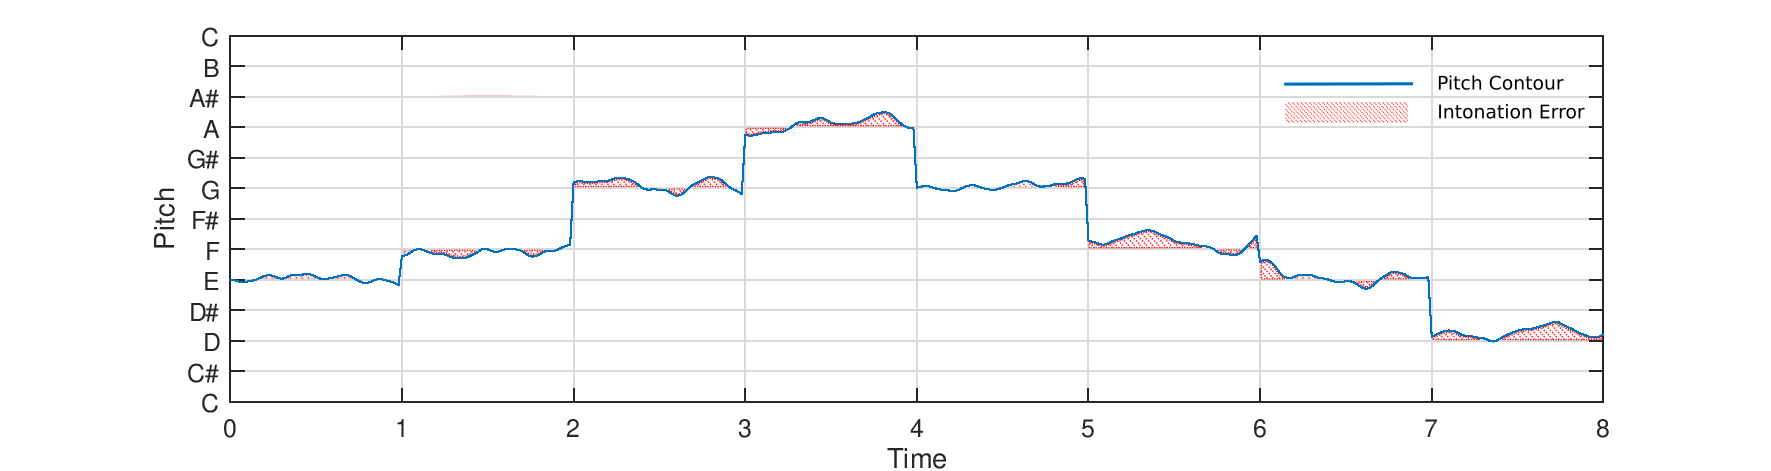
\includegraphics[width=\textwidth,trim={3.5cm 0cm 2.8cm 0cm}]
	{IntonationError}
	\caption{Illustration of Intonation Errors in a Pitch Contour Diagram}
	\label{fig:ErrorFunction}
\end{figure}

The red regions in figure \ref{fig:ErrorFunction} are intonation errors. To be
perfectly in tune would be saying there are no red regions, or equivalently, the
error function is zero everywhere. Therefore the smaller the red regions are the
better the pitch corrector. A common metric to measure this is the mean square
error metric and even has a built-in function in octave. Therefore the mean square
error would indicate how in tune the audio recording is, weighing larger
intonation errors greater than small intonation errors. This metric is referred to
as the mean squared pitch error and can fundamentally not be greater than
$1.736\times10^{-3}$ in the equal tempered tuning system. How this number is
calculated is shown in equation \ref{eq:MaxIntonationError} and is essentially
half the distance between two notes in the logarithmic pitch scale.

\begin{equation}\label{eq:MaxIntonationError}
	\bigg(\frac{1}{2}log_2(\sqrt[12]{2}) - log_2(1)\bigg)^2 \approx
	1.736\times10^{-3}
\end{equation}

To formalise this metric algorithm, a standard recording needs to be chosen to
test with. An exponential chirp signal is chosen, starting at 110Hz, ending at
440Hz and lasting 5 seconds. Figure \ref{fig:ChirpContour} shows the pitch contour
of the signal with the closest correct pitch contour. This signal has a mean
squared pitch error of $0.59 \times 10^{-3}$. The algorithm will measure the
mean squared pitch error after the pitch correction is applied and return a ratio
of the original and corrected mean squared pitch error. The idea being that the
metric essentially says the pitch correction effect causes the recording to be X
times more in tune. The goal of the pitch corrector is to maximise this metric.

\begin{figure}[h]
	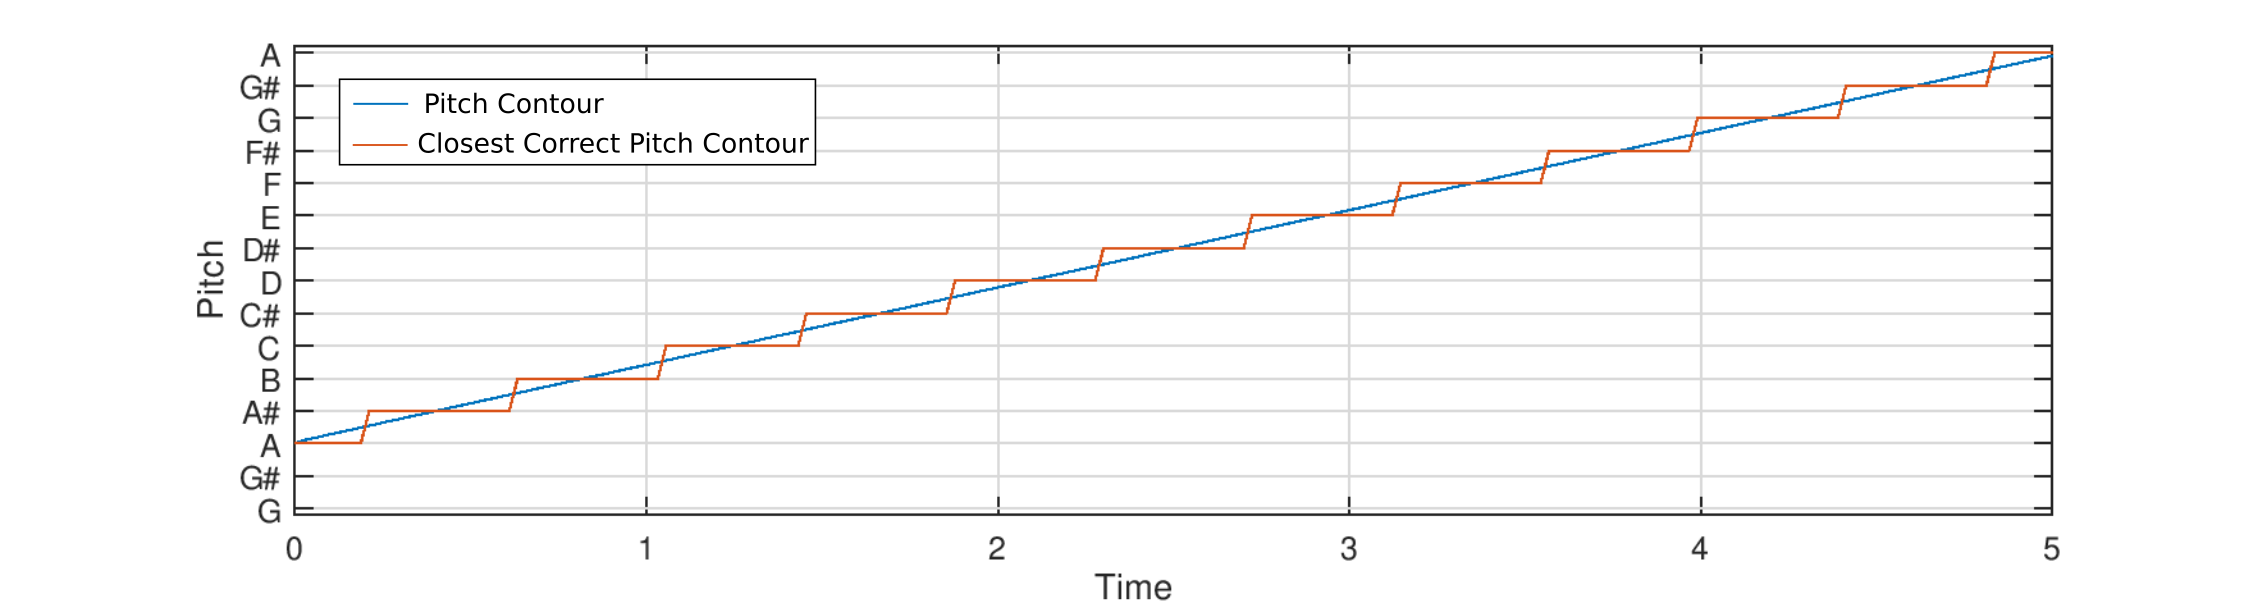
\includegraphics[width=\textwidth,trim={3.5cm 0cm 2.8cm 0cm}]
	{ChirpContour}
	\caption{Exponential Chirp Contour with Closest Frequency Contour}
	\label{fig:ChirpContour}
\end{figure}

The effectiveness metric unfortunately relies on the frequency detector to be
absolutely correct. This is because it depends on the results of the frequency
contour before and after the correction was made. The choice to use a clean chirp
signal for this metric was made to minimise dependence on the frequency detector.

Now that the effectiveness of the pitch corrector can be measured, a distortion
metric needs to be designed to measure how much the pitch corrector distorts the
signal unnecessarily. The idea is to have a signal in a state that it shouldn't
require a correction anymore, i.e. Already pitch corrected, and then apply the
pitch correction effect and see how much the signal change. The idea is to measure
the peak of the autocorrelation of a signal after applying the pitch correction
effect. This is the baseline value. Then apply the pitch correction effect again
and calculate the maximum value of the cross-correlation between the signal before
and after the second pitch correction effect has been applied. The ratio between
the maximum cross-correlation value and the baseline value gives in indication to
how much the pitch corrector distorts the signal unnecessarily. This ratio is
called the distortion metric, measured as a percentage. A pitch correction
algorithm will attempt to produce the highest similarity ratio, 100\% being a
perfect score. Listing \ref{lst:distortionMetric} shows the distortion metric
algorithm implemented in Octave.

\octavelisting{distortionMetric}

The testing recording for the distortion metric is chosen to be the same as the
one for the effectiveness metric except for one thing. The distortion signal needs
some added white noise to have the distortion in the whole frequency range
accounted for. To avoid the white noise from interfering with the frequency
detector, the level is set to \color{red}XX\color{black}db since both the
detectors are shown to be robust enough to that level of noise in the next
section.

\subsection{Noise Robustness Metric}

As has already been mentioned, the effectiveness metric relies on the fact that
the frequency detector is absolutely correct. To give some sense that the
frequency detector is capable of producing valid results, a metric is designed to
measure how much noise the frequency detector can deal with before producing
unacceptable results. Unacceptable results are seen as a mean square error of more
than $0.59 \times 10^{-6}$, i.e. three orders of magnitude greater than the mean
squared error of the testing signal in figure \ref{fig:ChirpContour}.

\color{red}
To Do:
\begin{itemize}
	\item Describe Frequency Detection Metric
	\item For a sense of completeness: Frequency scaling metric
	\item Describe Frequency Scaling metric
\end{itemize}
\color{black}

\section{Pitch Correction Design}

\color{red}
To do:
\begin{itemize}
	\item Touch on subsections and why each needs a section
\end{itemize}
\color{black}

\subsection{Structure}

\color{red}
To do:
\begin{itemize}
	\item Segmentation!!!
	\begin{itemize}
		\item Describe what segmentation is and why it is necessary
		\item Describe stages
		\begin{itemize}
			\item Split (overlap)
			\item Do computation
			\item Stitch (overlap and add)
		\end{itemize}
		\item Reason to overlap and size of overlapping (TRADE-OFF)
		\item Window size (TRADE-OFF)
		\begin{itemize}
			\item Small means low resolution
			\item Large means latency
			\item Small generally means more computation
		\end{itemize}
		\item Properties to preserve relevant to real time auto tuning
	\end{itemize}
	\item Flow diagram
	\item Actual code snips from Octave source code
\end{itemize}
\color{black}

\subsection{Interface}

\color{red}
To do:
\begin{itemize}
	\item Interface philosophy
	\item Frequency detectors and scalers should be swappable
\end{itemize}
\color{black}

\section{Choosing Wanted Frequency}

\color{red}
To do:
\begin{itemize}
	\item Describe why choosing wanted frequency is not trivial
	\item Naive approach
	\begin{itemize}
		\item Describe approach
		\item Show results of approach
	\end{itemize}
	\item Schmitt Trigger Approach
	\begin{itemize}
		\item Describe approach
		\item Show results of approach
	\end{itemize}
	\item Evaluation Metric
	\begin{itemize}
		\item Describe metric
		\item Show why Schmitt trigger is better
	\end{itemize}
\end{itemize}
\color{black}

\section{Frequency Detector}

\color{red}
To do:
\begin{itemize}
	\item Explain that this is the basis for the frequency scaler
	\item Explain other things
\end{itemize}
\color{black}

\subsection{Zero Crossing Method}

\color{red}
To do:
\begin{itemize}
	\item Describe method in more detail than lit review
	\item Show snips of code and graphically what it's doing
	\item Show performance metrics
\end{itemize}
\color{black}

\subsection{Autocorrelation Method}

\color{red}
To do:
\begin{itemize}
	\item Describe method in more detail than lit review
	\item Show snips of code and graphically what it's doing
	\item Show performance metrics
\end{itemize}
\color{black}

\section{Frequency Scaler}

\color{red}
To do:
\begin{itemize}
	\item Explain time vs frequency approaches
	\item Explain other things
\end{itemize}
\color{black}

\subsection{Phase Vocoder}

\color{red}
To do:
\begin{itemize}
	\item Describe method in more detail than lit review
	\item Show snips of code and graphically what it's doing
	\item Show performance metrics
\end{itemize}
\color{black}

\subsection{Simple Overlap and Add}

\color{red}
To do:
\begin{itemize}
	\item Describe method in more detail than lit review
	\item Show snips of code and graphically what it's doing
	\item Show performance metrics
\end{itemize}
\color{black}

\section{Pitch Corrector}

\color{red}
To do:
\begin{itemize}
	\item Describe which modules were added put together
	\item Describe why each module was chosen
	\item Describe each system and show its performance
\end{itemize}
\color{black}

\section{Concept Expansion}

\color{red}
To do:
\begin{itemize}
	\item Explain that more cool stuff were found
	\item Post Correction
	\item Harmonization
	\item Pitch Scaling by a Constant Factor
\end{itemize}
\color{black}
